\documentclass{exam-zh}
\usepackage{siunitx}

\examsetup{
  page/size=a4paper,
  paren/show-paren=true,
  paren/show-answer=true,
  fillin/show-answer=false,
  solution/show-solution=show-stay,
  solution/label-indentation=false
}


\everymath{\displaystyle}

\title{2024 年森铭中学第一学期期末考试}

\subject{挠痒理论}



\begin{document}

% \information{
%   姓名\underline{\hspace{6em}},
%   座位号\underline{\hspace{15em}}
% }
% \warning{(在此卷上答题无效)}

\secret

\maketitle

本试卷共 6 页,37 题。全卷满分 150 分。考试用时 150 分钟。


\begin{notice}
  \item 答题前,先将自己的姓名、准考证号、考场号、座位号填写在试卷和答题卡上,
    并将准考证号条形码粘贴在答题卡上的指定位置。
  \item 选择题的作答:每小题选出答案后,用 2B 铅笔把答题卡上对应题目的答案标号涂黑。
    写在试卷、草稿纸和答题卡上的非答题区域均无效。
  \item 填空题和解答题的作答:用黑色签字笔直接答在答题卡上对应的答题区域内。
    写在试卷、草稿纸和答题卡上的非答题区域均无效。
  \item 考试结束后,请将本试卷和答题卡一并上交。
\end{notice}



\section{%
  视频题:本题共 10 小题,每小题 2 分,共 20 分。
  在每小题给出的四个选项中,只有一项是符合题目要求的。
}

观看视频1,回答问题1-4


\begin{question}[points = 2]
  视频中出现的挠痒方式为



  \begin{choices}
    \item X型捆绑
    \item 悬挂式捆绑
    \item 座椅捆绑
    \item 脚踝捆绑
  \end{choices}
\end{question}

\begin{question}[points = 2]
  视频中哪种挠痒手法没有出现



  \begin{choices}
    \item 双手异步技巧
    \item 快速点触法
    \item 循环旋转法
    \item 隔空假动作
  \end{choices}
\end{question}

\begin{question}[points = 2]
  视频显示,被挠者最敏感的区域似乎是



  \begin{choices}
    \item 脚心
    \item 腰肋
    \item 大腿
    \item 脖子
  \end{choices}
\end{question}

\begin{question}[points = 2]
  被挠者尝试使用哪种防御策略?



  \begin{choices}
    \item 身体扭动
    \item 用手护住敏感区域
    \item 口头请求停止
    \item 口头请求停止
  \end{choices}
\end{question}


观看视频2,回答问题5-10

\begin{multifigures}
\item[ 红色被挠裤 ] 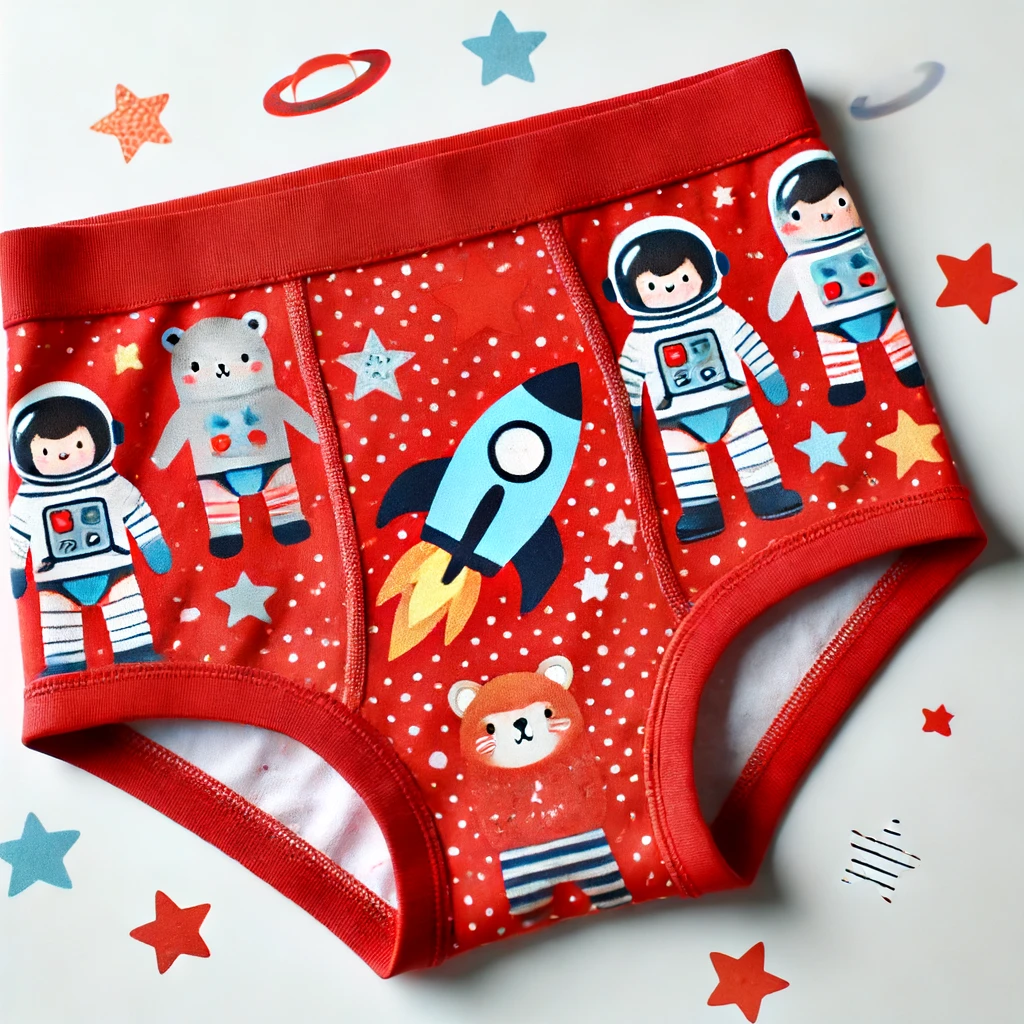
\includegraphics [width =3cm]{ red.png}
\item[ 白色被挠裤 ] 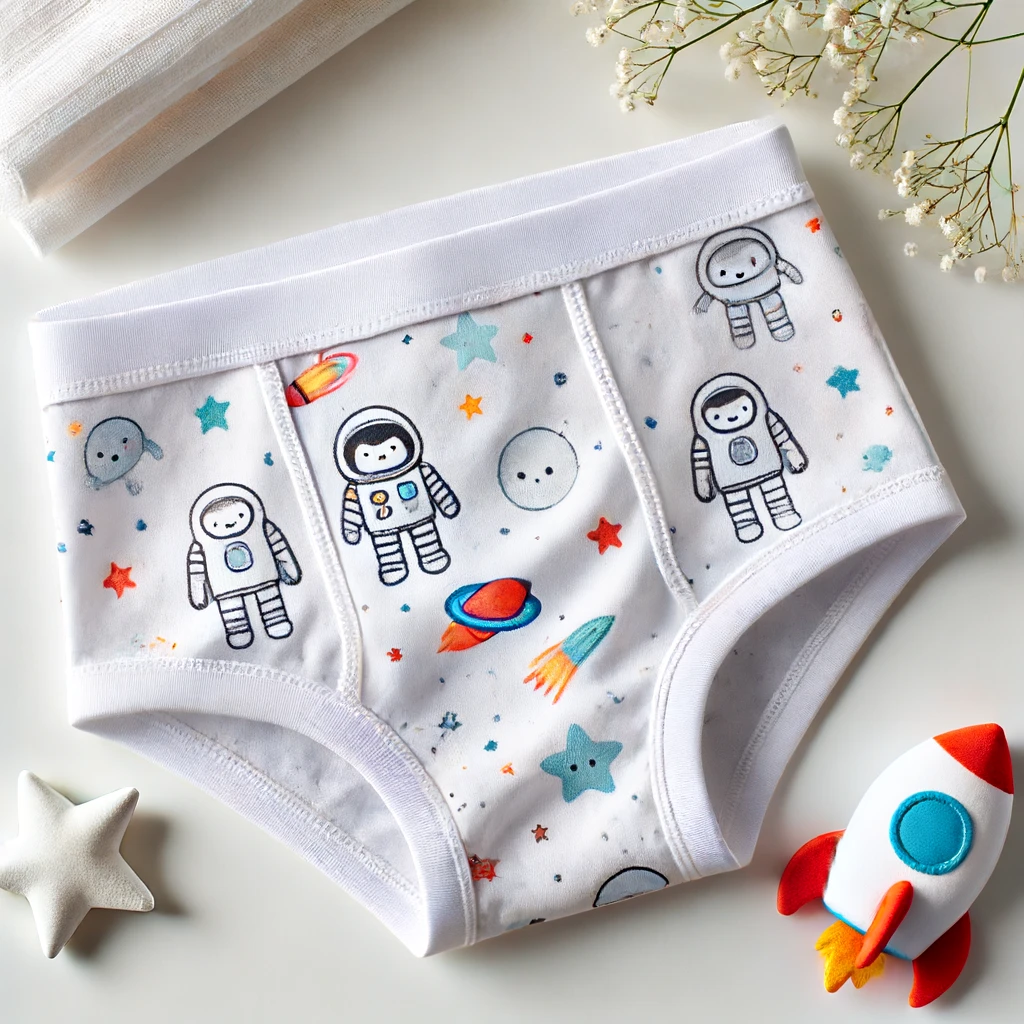
\includegraphics [width =3cm]{ white.png}
\end{multifigures}

\begin{question}[points = 2]
  视频中两位参与者主要采用了哪种挠痒痒策略?



  \begin{choices}
    \item 单点持续攻击
    \item 快速多点切换
    \item 混合使用多种技巧
    \item 使用虚招混淆对手
  \end{choices}
\end{question}


\begin{question}[points = 2]
  根据视频,哪个敏感区域被频繁利用?



  \begin{choices}
    \item 腋下
    \item 脚底
    \item 肋骨
    \item 腰部
  \end{choices}
\end{question}

\begin{question}[points = 2]
  视频有红框显示的时间内,红色被挠裤的挠痒者对于对手使用的战术是



  \begin{choices}
    \item 反向交替法
    \item 温柔交替法
    \item 循环旋转法
    \item 双手异步法
  \end{choices}
\end{question}

\begin{question}[points = 2]
  视频显示,哪位参与者的笑声和反应更为强烈?



  \begin{choices}
    \item 红色被挠裤
    \item 白色被挠裤
    \item 两者反应相似
    \item 视频中无法确定
  \end{choices}
\end{question}

\begin{question}[points = 2]
  视频显示,哪位参与者更频繁地使用心理战术,如假动作或虚晃?  


  \begin{choices}
    \item 红色被挠裤
    \item 白色被挠裤
    \item 两者反应相似
    \item 视频中无法确定
  \end{choices}
\end{question}

\begin{question}[points = 2]
  视频中哪位参与者获得了最终胜利?



  \begin{choices}
    \item 红色被挠裤
    \item 白色被挠裤
    \item 平局
    \item 视频中无法确定
  \end{choices}
\end{question}



\section{%
  选择题:本题共 8 小题,每小题 2 分,共 16 分。
  在每小题给出的四个选项中,只有一项是符合题目要求的。
}


\begin{question}[points = 2]
  哪个区域通常不被视为挠痒痒的常规敏感区域?



  \begin{choices}
    \item 脖子
    \item 腰部
    \item 脚底
    \item 前臂
  \end{choices}
\end{question}
% 1.
\begin{question}[points = 2]
  如果挠痒痒的总时间取决于初始痒感强度、敏感度系数和抗痒能力,当抗痒能力增强时,总时间会如何变化?

  \begin{choices}
    \item 增加
    \item 减少
    \item 保持不变
    \item 先增加后减少
  \end{choices}
\end{question}

\begin{question}[points = 2]
  笑声的响度是由哪两个因素决定的?

  \begin{choices}
    \item 挠痒痒的强度和时间
    \item 痒点数量和被挠面积
    \item 手臂质量和速度
    \item 挠痒痒的频率和时间
  \end{choices}
\end{question}

\begin{question}[points = 2]
  挠痒痒最常用的手指技巧是什么?

  \begin{choices}
    \item 轻弹
    \item 揉搓
    \item 轻划
    \item 捏抓
  \end{choices}
\end{question}



\begin{question}[points = 2]
  在挠痒痒大战中,如何判定胜负?

  \begin{choices}
    \item 时间最长的一方胜出
    \item 让对方笑声最大的一方胜出
    \item 第一个停止的一方胜出
    \item 让对方先说“停”的一方胜出
  \end{choices}
\end{question}

\begin{question}[points = 2]
  当挠痒痒的速度加倍时,消耗的能量如何变化?

  \begin{choices}
    \item 不变
    \item 四倍
    \item 减半
    \item 加倍
  \end{choices}
\end{question}

\begin{question}[points = 2]
  当手指移动的长度减少一半时,挠痒痒的频率会

  \begin{choices}
    \item 不变
    \item 四倍
    \item 减半
    \item 加倍
  \end{choices}
\end{question}


\begin{question}[points = 2]
  当痒点密度$P(x,y)$在中心点最高时,痒点覆盖率 $R$ 的变化将指示什么?

  \begin{choices}
    \item 覆盖率和痒感都增加

    \item 覆盖率增加,但痒感减少
    \item 覆盖率减少,但痒感增加
    \item 覆盖率和痒感都减少
  \end{choices}
\end{question}









\section{填空题:本题共 5 小题,每小题 3 分,共 15 分。}


\begin{question}
  挠痒的四种基本指法分别为:戳,捏, \fillin[$1$],抓 。
\end{question}

\begin{question}
  挠痒中眼罩的作用是\fillin[$2$] 。
\end{question}

\begin{question}
  迅速而轻柔地在对方身体的多个敏感区域(如腋下和脚底)轻点,类似钢琴手的手法,迅速转换挠痒痒的位置的方法称作 \fillin[$1$]。
\end{question}

\begin{question}
  在挠痒实战中,更多用到的技巧是\fillin[$1$](“时间差挠痒”或“反向交替挠痒”) 。
\end{question}

\begin{question}
  在一次挠痒痒活动中,如果初始痒感强度为10,敏感度系数为3,而抗痒能力为2,则根据挠痒痒时长公式,总时间是 \fillin[$1$] 秒。
\end{question}


\begin{question}
  如果四个手指共同作用,手指移动长度为$10 {cm}$,被挠面积为$50 {cm}^2$,挠痒痒的频率为  \fillin[$1$] Hz。
\end{question}


\section{实验题:本题共 4 小题,共 21 分。}


\textbf{实验大题:挠痒工具对不同敏感区域的影响}

你作为一名研究人员,正在研究不同挠痒工具对人体不同敏感区域的影响。你将进行一个实验,以探讨手指、羽毛挠痒棒和电动挠痒工具在腋下、脚底和颈部这三个敏感区域的效果。实验的目的是测量每种工具在每个敏感区域引起的反应时间和主观感受,并进行数据分析以确定不同工具和区域之间的关系。

\textbf{实验材料}: 手指, 羽毛挠痒棒, 电动挠痒工具, 计时器, 笑声响度记录表, 问卷调查表(用于记录主观感受), 志愿者(10人,14岁、不同性别)

\textbf{实验步骤}:
\begin{step}
\item 每次分别使用手指、羽毛挠痒棒、电动挠痒工具进行实验。
\item 在控制的环境下进行实验,确保每次实验的持续时间和力度一致。
\item 在志愿者的腋下、脚底和颈部分别进行挠痒,每次持续10秒。
\item 使用计时器记录从挠痒开始到志愿者开始笑或表现出明显不适的时间。
\item 记录每位志愿者对不同工具和不同敏感区域的反应时间和主观感受(通过问卷调查)。
\item 重复实验,确保数据的可靠性。
\item 数据分析
\end{step}
\begin{problem}[points = 5]实验设计与数据记录
  \begin{enumerate}
    \item 描述如何使用计时器和记录表来精确记录每次实验中的笑声响度。

    \item {假设手指、羽毛和电动工具分别引起以下笑声响度:
    \begin{table}[h]
      \centering
      \begin{tabular}{|c|c|c|c|c|c|c|c|c|c|c|}
      \hline
       & 小明 & 小红 & 小华 & 小丽 & 小刚 & 小芳 & 小杰 & 小霞 & 小强 & 小梅 \\
      \hline
      手指 & 5.2 & 6.0 & 5.8 & 6.2 & 5.5 & 6.1 & 5.9 & 6.3 & 5.7 & 6.0 \\
      \hline
      羽毛 & 6.5 & 7.0 & 6.8 & 7.2 & 6.9 & 7.1 & 6.7 & 7.3 & 6.6 & 7.0 \\
      \hline
      电动工具 & 4.8 & 5.1 & 5.0 & 4.9 & 5.3 & 5.2 & 5.0 & 5.4 & 5.1 & 5.0 \\
      \hline
      \end{tabular}
      \end{table}
    \newline 计算每种工具的平均笑声响度和挠痒痒的强度,并解释这些结果的物理意义。}

    \begin{table}[h]
      \centering
      \begin{tabular}{|c|c|c|c|}
      \hline
       & 手指 & 羽毛 & 电动工具 \\
      \hline
      平均笑声响度 & \fillin[$1$] & \fillin[$1$] & \fillin[$1$] \\
      \hline
      挠痒痒的强度 & \fillin[$1$] & \fillin[$1$] & \fillin[$1$] \\
      \hline
      \end{tabular}
      \end{table}


  \end{enumerate}
 
\end{problem}


\begin{question}
  小明的敏感度系数比小红\fillin[$1$](“高”或“低”) 。
\end{question}

\begin{question}
  小明的抗痒能力比小华 \fillin[$1$](“高”或“低”) 。
\end{question}



\begin{problem}[points = 5]实验结果与讨论
  \begin{enumerate}
    \item 根据实验数据,讨论哪种工具对大多数志愿者产生了最强的挠痒反应,并提供可能的生理或心理解释。

    \item 分析是否存在显著的年龄或性别差异,结合实验数据讨论不同人群对特定工具的敏感性。


  \end{enumerate}
 
\end{problem}


\begin{problem}[points = 5]改进与扩展
  \begin{enumerate}
    \item 提出改进实验设计的建议,例如如何增加数据的可靠性和准确性。

    \item 设想一个扩展实验,研究其他类型的刺激(如温度变化或震动)对挠痒敏感度的影响,你的研究方向为 \fillin[width = 2cm][$1$]。


  \end{enumerate}
 
\end{problem}


\section{材料题:本题共 7 小题,共 26 分。}

\begin{material}[author = 杨宇, title = { 小智的故事 }]
“嘿,小智,我们玩个游戏吧!”小明笑着提议,眼中闪烁着狡黠的光芒。其他朋友们也随声附和,纷纷表示赞同。小智有些疑惑,但也没有多想,毕竟都是多年的好友,玩个游戏应该没什么大不了的。

然而,当他被五花大绑地固定在床上时,小智意识到事情并没有他想的那么简单。朋友们用柔软的绳子牢牢地捆住了他的手脚,确保他无法挣脱。小智挣扎了一下,发现自己动弹不得,心里顿时涌起了一股不安。

“你们要干什么?”小智有些紧张地问道,声音里带着一丝颤抖。

“放心,小智,我们只是想给你点特别的惊喜。”小明神秘地笑了笑,手中拿出了一根羽毛。

小智看到那根羽毛,顿时明白了他们的意图。他想起了几次和朋友们的玩笑话,自己提到过非常怕痒。现在,这个弱点成了朋友们的目标。

小明慢慢地把羽毛靠近小智的脚底,那根轻盈的羽毛仅仅是触碰到他的皮肤,小智就感到一阵电流般的痒意迅速传遍全身。“哈哈哈,不行,不行,别挠我!”小智忍不住大笑起来,整个身体因为痒感而微微颤抖。

“这才刚开始呢,小智!”小丽也加入了进来,她手中拿着一把软刷子,开始在小智的腰侧轻轻刷动。腰部是小智的另一个敏感区,刷子的轻触让他笑得更加厉害,身体拼命地扭动着试图避开那些痒感,但根本无法成功。

“哈哈哈,求求你们,停下,哈哈哈,太痒了!”小智的笑声不断,他的脸因为持续的大笑而变得通红,眼角甚至流出了笑泪。每一次的触碰都像是无数的小虫在皮肤上爬行,痒得他几乎要失去理智。

朋友们没有停下,他们似乎乐在其中,不断变换着挠痒的方式。羽毛在脚底来回滑动,刷子在腰侧轻轻刷着,有人甚至用手指在他的腋下和肋骨间快速挠动。每一个动作都精准地命中小智的痒点,带来无尽的痒意。

小智的笑声逐渐变得嘶哑,他的呼吸也变得急促。尽管身体已经被绑得动弹不得,但他依然拼命挣扎,试图躲开那些令人难以忍受的挠痒。痒感像潮水一样一波接一波地袭来,压得他喘不过气来。

“哈哈哈,求你们了,停下吧,我受不了了!”小智几乎是在乞求,但朋友们显然还没玩够。他们继续变换着挠痒的节奏和力度,让小智的每一根神经都在痒感中绷紧。

随着时间的推移,小智的身体逐渐变得无力,笑声也从开始的爽朗变成了疲惫的喘息。但即使如此,每一次的挠痒依然能激起他身体深处的痒意,让他无法停止挣扎和大笑。

就在他以为自己快要失去理智的时候,朋友们开始变换挠痒的方式。小明拿出了一个电动按摩器,调整到最低档位,然后轻轻地在小智的脚底滑动。微微震动的按摩头让小智感受到一种全新的痒感,比刚才的羽毛和刷子更加深入。

“哈哈哈,不要,不要这样,哈哈哈!”小智几乎要哭出来了,他的脚趾紧紧蜷缩,想要躲避这种奇怪的感觉,却无能为力。

与此同时,小丽换上了一根带有软橡胶刷头的小棒,轻轻地在小智的腋下来回刷动。软橡胶刷头的触感比手指更加细腻,每一次刷动都像是无数只小虫在他的皮肤上爬行,让小智痒得几乎要爆炸。

“哈哈哈,哈哈哈,我不行了,哈哈哈,停下来!”小智的笑声混杂着喘息,脸上因为持续的大笑而变得通红,眼角流出了笑泪。

小刚也加入了进来,他手中拿着一根长长的羽毛,轻轻地在小智的肋骨间滑动。羽毛的轻柔触感让小智的每一根神经都绷紧了,每一次轻触都引发一阵阵的痒意,让他更加无法忍受。

“哈哈哈,哈哈哈,求求你们,哈哈哈,停下,哈哈哈,太痒了!”小智的声音已经沙哑,身体因为痒感而剧烈扭动着,但他无论如何也挣脱不了那些柔软的束缚。

朋友们似乎玩得越发起劲,他们继续变换着挠痒的方式。小华拿出了一根带有小刷子的挠痒棒,刷头上涂了少量润滑剂,使刷子的移动更加顺滑。她轻轻地在小智的脖子后面和耳朵周围挠动,敏感的皮肤立刻传来一阵阵的痒感,像是无数小电流在皮肤下流动。

“哈哈哈,哈哈哈,不要,哈哈哈,我快要疯了,哈哈哈!”小智的笑声断断续续,整个人已经被痒感折磨得筋疲力尽,但朋友们并没有停下的意思。

最后,小龙拿出了一个带有多个触角的电动挠痒器,这些触角可以在不同的方向同时移动。小龙将它放在小智的腹部,让触角轻轻地挠动他的皮肤。腹部是小智最为敏感的地方之一,这种多点同时挠动的感觉让他瞬间崩溃。

“哈哈哈,哈哈哈,哈哈哈,停下来,哈哈哈,我受不了了,哈哈哈!”小智的笑声几乎变成了哭声,身体在床上剧烈扭动,仿佛要挣脱一切。

朋友们看到小智已经到了极限,终于停下了手中的动作。他们解开了小智的束缚,看着他大口喘着气,脸上满是汗水和泪水,身体因为疲惫而微微颤抖。




\end{material}


% 18.
\begin{question}[points = 2]
  朋友们使用电动按摩器和带有润滑剂的小刷子来挠痒小智,这些工具主要是为了达到什么效果?
  \begin{choices}
    \item 增强痒感的深度和复杂性
    \item 让小智感到舒适和放松
    \item 测试小智的耐力和抗痒能力
    \item 分散小智的注意力
  \end{choices}
\end{question}


\begin{question}[points = 2]
  当小智的朋友们使用不同的挠痒方式时,哪种方式对小智产生了最强烈的反应?
  \begin{choices}
    \item 手指轻挠脚底
    \item 羽毛滑动肋骨
    \item 电动挠痒器在腹部多点同时挠动
    \item 软橡胶刷头刷动腋下
  \end{choices}
\end{question}

\begin{question}[points = 2]
  小智被朋友们挠痒时,哪种挠痒工具在他的颈部和耳朵周围使用效果最佳?
  \begin{choices}
    \item 羽毛
    \item 手指
    \item 电动按摩器
    \item 带有软橡胶刷头的小棒
  \end{choices}
\end{question}

\begin{problem}[points = 5]分析小智在不同挠痒工具和方法下的反应,结合我们之前讨论的挠痒敏感度与刺激类型的关系,解释为什么这些工具能引发强烈的痒感。\end{problem}

\begin{problem}[points = 5]朋友们使用了哪些具体的挠痒技巧(如双手异步技巧、虚实结合等)来增加小智的痒感?请结合文章细节具体说明。\end{problem}

\begin{problem}[points = 5]  小智在被朋友们挠痒时的身体和心理反应经历了哪些阶段?结合我们之前聊过的挠痒生理和心理效应,详细描述这些变化。\end{problem}

\begin{problem}[points = 5]  在朋友们使用电动挠痒器时,小智的反应特别强烈,结合电动挠痒器的特点,解释为什么这种工具比手指或羽毛更有效。\end{problem}


\section{作文:50分}
\begin{material}
  “小智的朋友们不断变换挠痒的方法,羽毛轻抚、手指挠动、电动挠痒器多点同时作用,这些不同的刺激让小智几乎崩溃。每一次的挠痒都像是无数的小虫在他的皮肤上爬行,痒得他几乎要失去理智。”
\end{material}


\begin{problem}[points = 50] 请写一篇不少于500字的文章,描述你个人经历中使用特定挠痒工具的一次体验,并解释这种体验如何让你感受到小智在文章中的强烈反应。你可以详细描述工具的使用过程、你的感受和反应,以及这次经历给你留下的印象。\end{problem}


\end{document}